%\chapter{Bose--Einstein condensate dynamics}
\section{Condensate dynamics}
In the following section I will examine the dynamics of the condensate following two distinct perturbations. Firstly, I will discuss the application of an external potential to the trapped condensate for a short timescale. Next, I will directly manipulate the wavefunction phase. Though these two methods are physically implemented by similar means, they serve two very different purposes, and they will be treated as such.

\section{Simulating Bose--Einstein condensates}
In Sections ~\ref{sec:analytics,sec:numerics} I have outlined both analytical Thomas-Fermi (TF) and numerical solutions of the Gross--Pitaevskii equation. It is instructive to compare the results from these two methods. The profile and width should be comparable, with the TF solution deviating only in the low-density regions. Fig.~\ref{fig:gpe_tf_3} shows a comparison of the two-dimensional profile for both methods, showing good agreement, and hence a well developed numerical procedure.
\begin{figure}\centering
    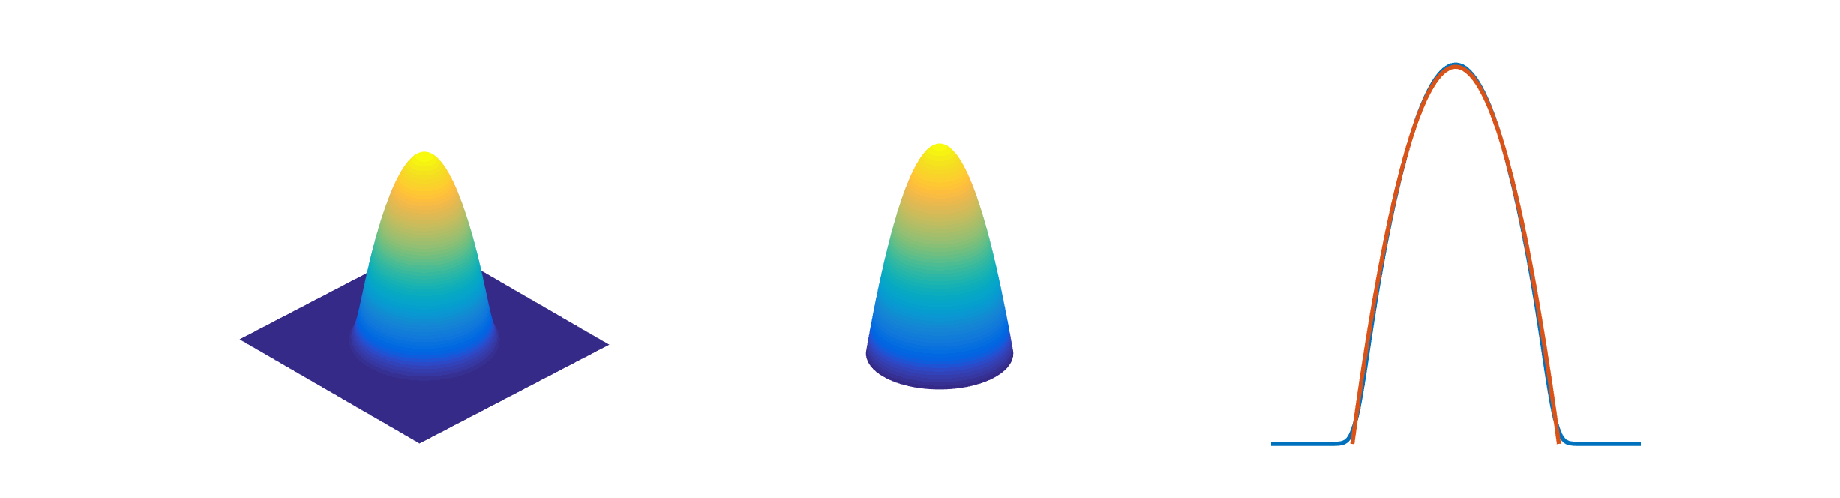
\includegraphics[width=\textwidth,trim=0ex 0ex 0ex 0ex]{Images/ch4_vtx/gpe_tf_3.pdf}
    \caption{The numerical solution (left) and Thomas-Fermi (middle) solutions for a two-dimensional condensate of $^{87}$Rb with $N=1\times 10^5$ atoms. The lineplot (right) is a central cut through both profiles showing the close match.}\label{fig:gpe_tf_3}
\end{figure}

While the Thomas--Fermi solution is a close agreement with the numerical solution of the Gross--Pitaevskii equation, this solution is only applicable for stationary states with negligible kinetic energy. For more complex problems involving dynamics, full numerical integration of the Gross--Pitaevskii equation is required. One such example is that of superfluid vortex dynamics. The numerical generation of a stable set of vortices in a Bose--Einstein condensate is achieved by solving the Gross--Pitaevskii equation Hamiltonian in the frame co-rotating with the condensate Eq.~\ref{eqn:}. To seed a single vortex in the condensate, the frequency of rotation, $\Omega$, must be higher than the critical rotation frequency $\Omega_c$, as discussed in Sec.~\ref{sec:}, and in the presence of dissipation to allow for energetic losses. Numerically, this is achieved by simulating the condensate in the co-rotating frame as given by Eq.~\ref{eqn:gpe_rotation} in imaginary time.

\lee{{!!!Need to fix this!!!]}


\section{Vortex lattice solutions}
To generate vortices in a BEC the energy of the condensate in the presence of a vortex at the required rotation rate must be lower than without. The rotation frequency should be greater than or equal to that of the critical rotation frequency for seeding a vortex, $\Omega \geq\Omega_c$, as given by Eq.~\ref{eqn:crit_rot}. For a linear ramp of the rotation frequency during imaginary time evolution, as discussed in Sec.~\ref{sec:linramp}, I essentially follow the groundstate solution at all times. This has an added advantage of returning a groundstate solution for any required rotation frequency, with the number of vortices increasing as higher frequencies are reached. An example of several states from a single simulation are given in Fig.~\ref{fig:inc_omega}. The previously discussed resolution considerations become apparent as the rotation rate is increased for both position and momentum space representations of the wavefunction. A sample movie of the generation is given here \cite{MLXD:movie_groundstates}, wherein I ramp the frequency from $\Omega/\omega_\perp = 0.39 \to 0.995$ and plot the wavefunction density $|\Psi(\mathbf{r},t)|$.

\begin{figure}\centering
    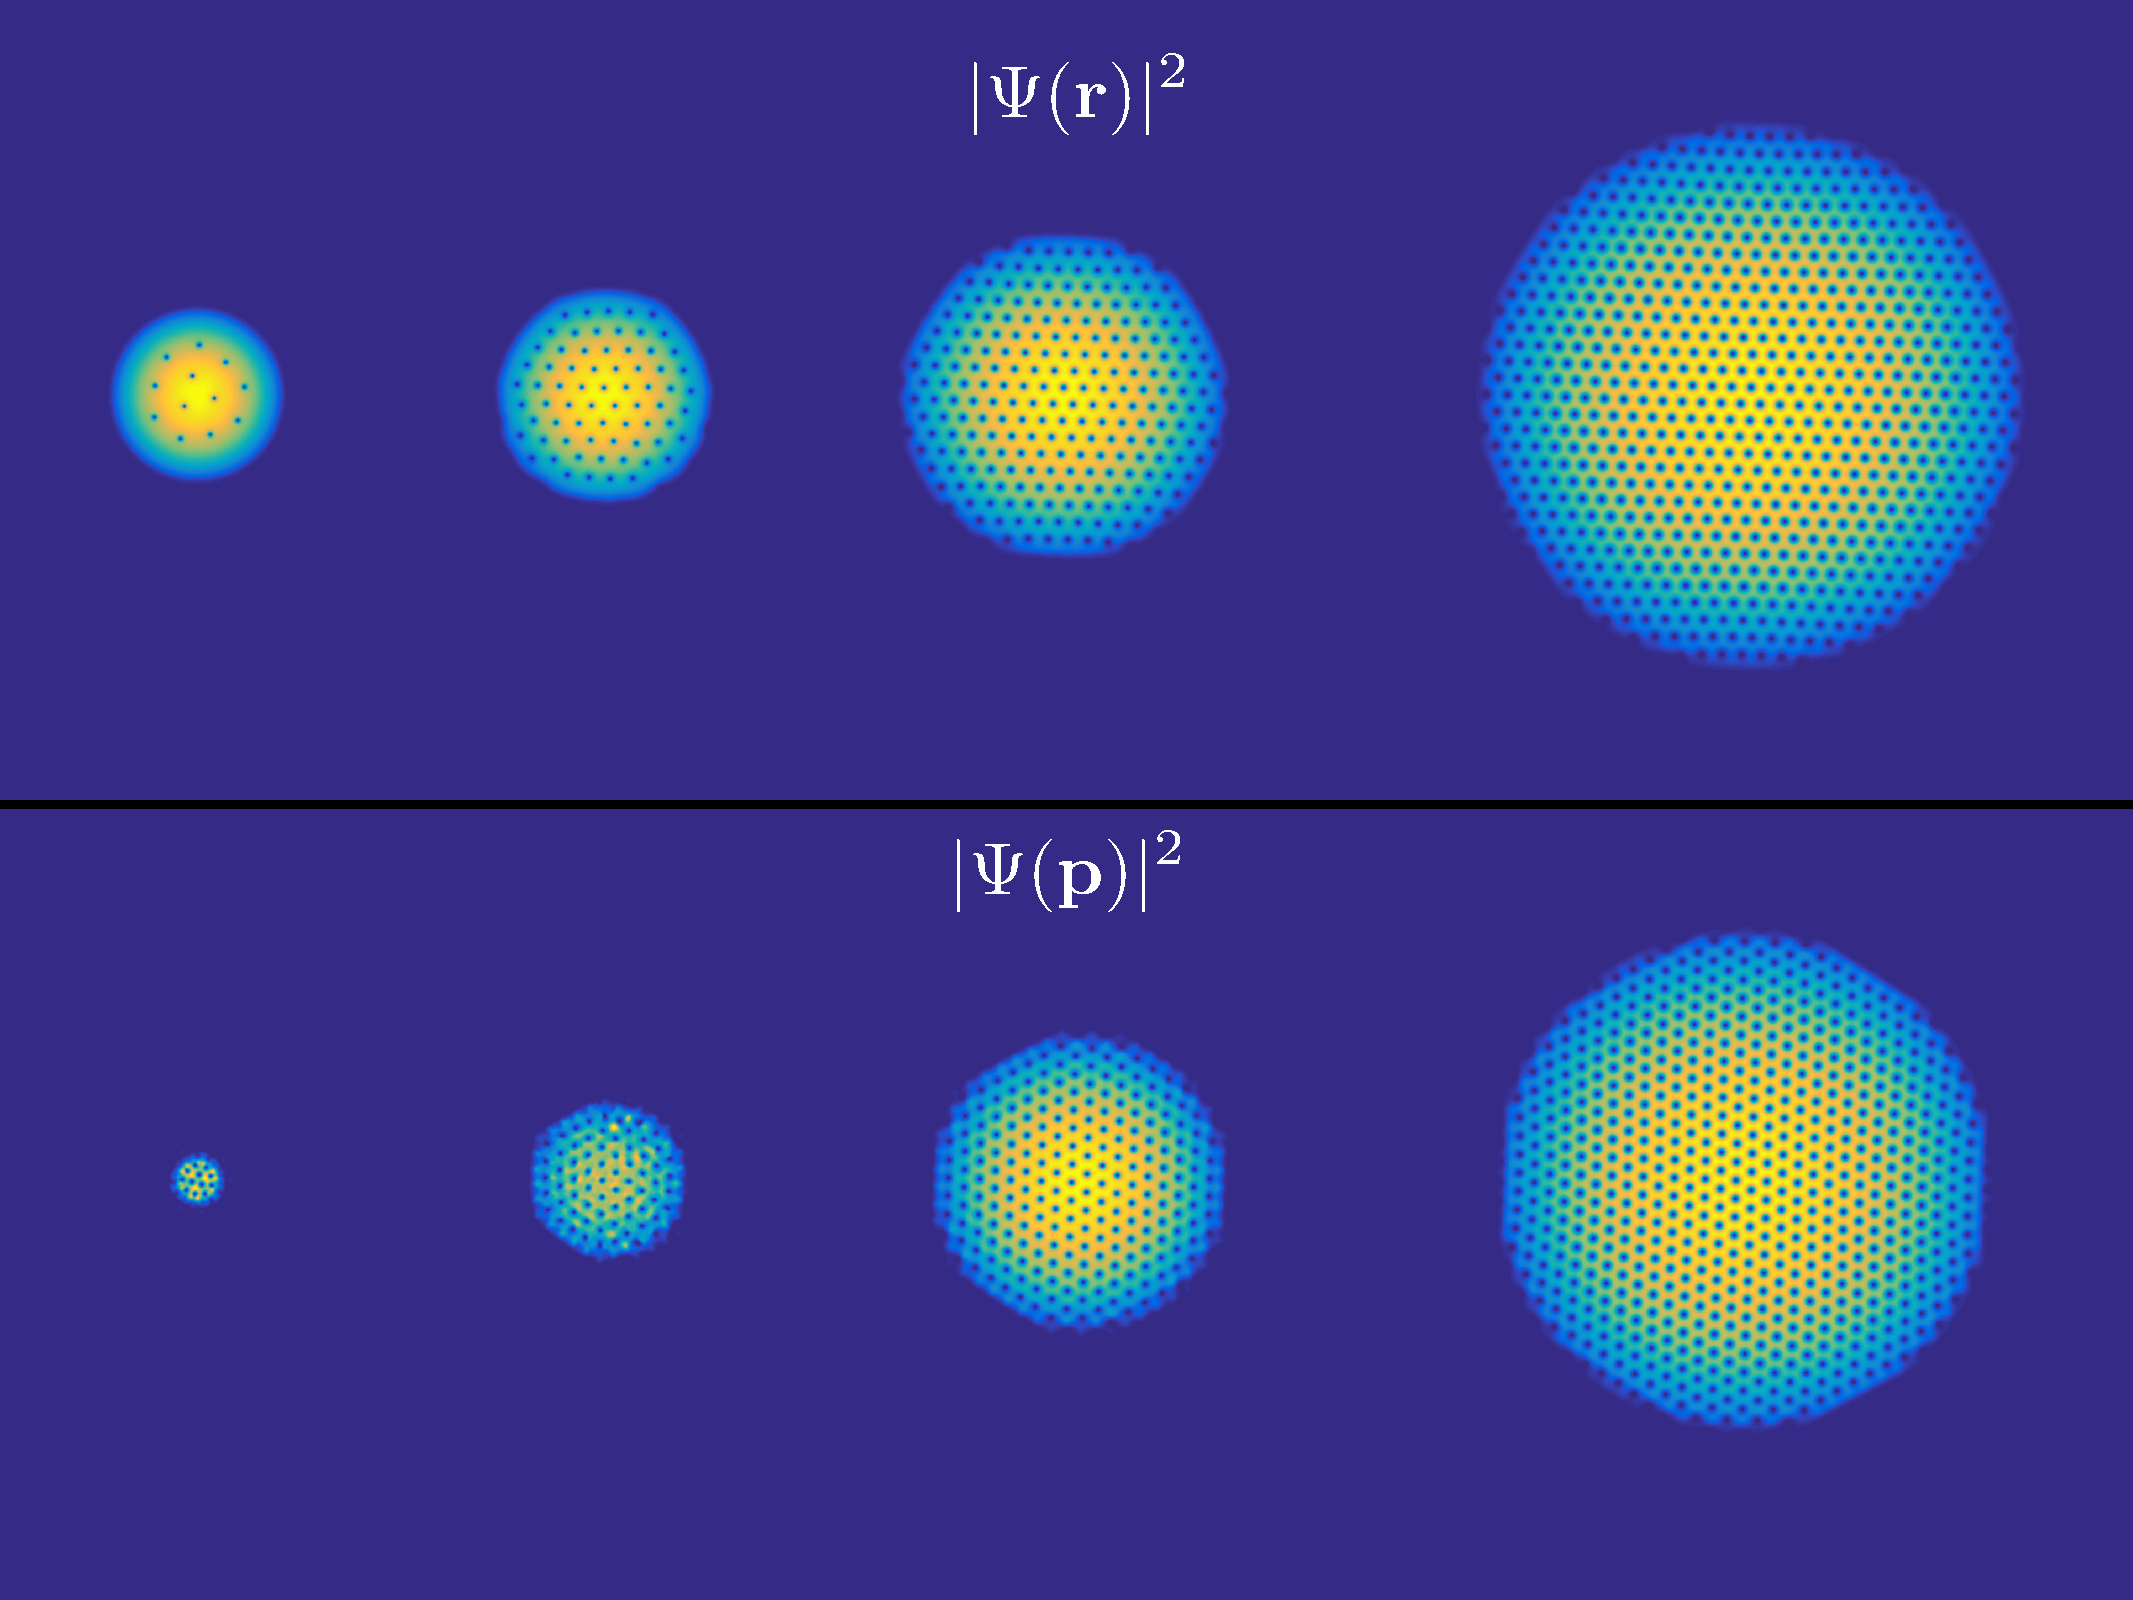
\includegraphics[width=0.85\textwidth]{Images/ch4_vtx/ramp_omega.pdf}
    \caption{The density distributions of the wavefunction in position (top) and momentum (bottom) space are given for rotation frequencies (L-R) $\Omega/\omega_\perp=[0.366,0.796,0.962,0.995]$. The color axis differs for each plot, as a constant axis is difficult to view densities across all magnitudes. The growth rate of the condensate radius in both position and momentum space becomes large when $\Omega \approx \omega_\perp$.}
    \label{fig:inc_omega}
\end{figure}

If the linear ramp is performed too quickly, or if I instantaneously choose a groundstate with a large amount of angular momentum, the vortices tend to enter from the boundary all at one instance, and fail to ever find a well ordered groundstate. An example of this such issue is given by Fig.~\ref{}, and indicates the need for a slow linear ramp that is essentially adiabatic in imaginary time.

\begin{figure}
    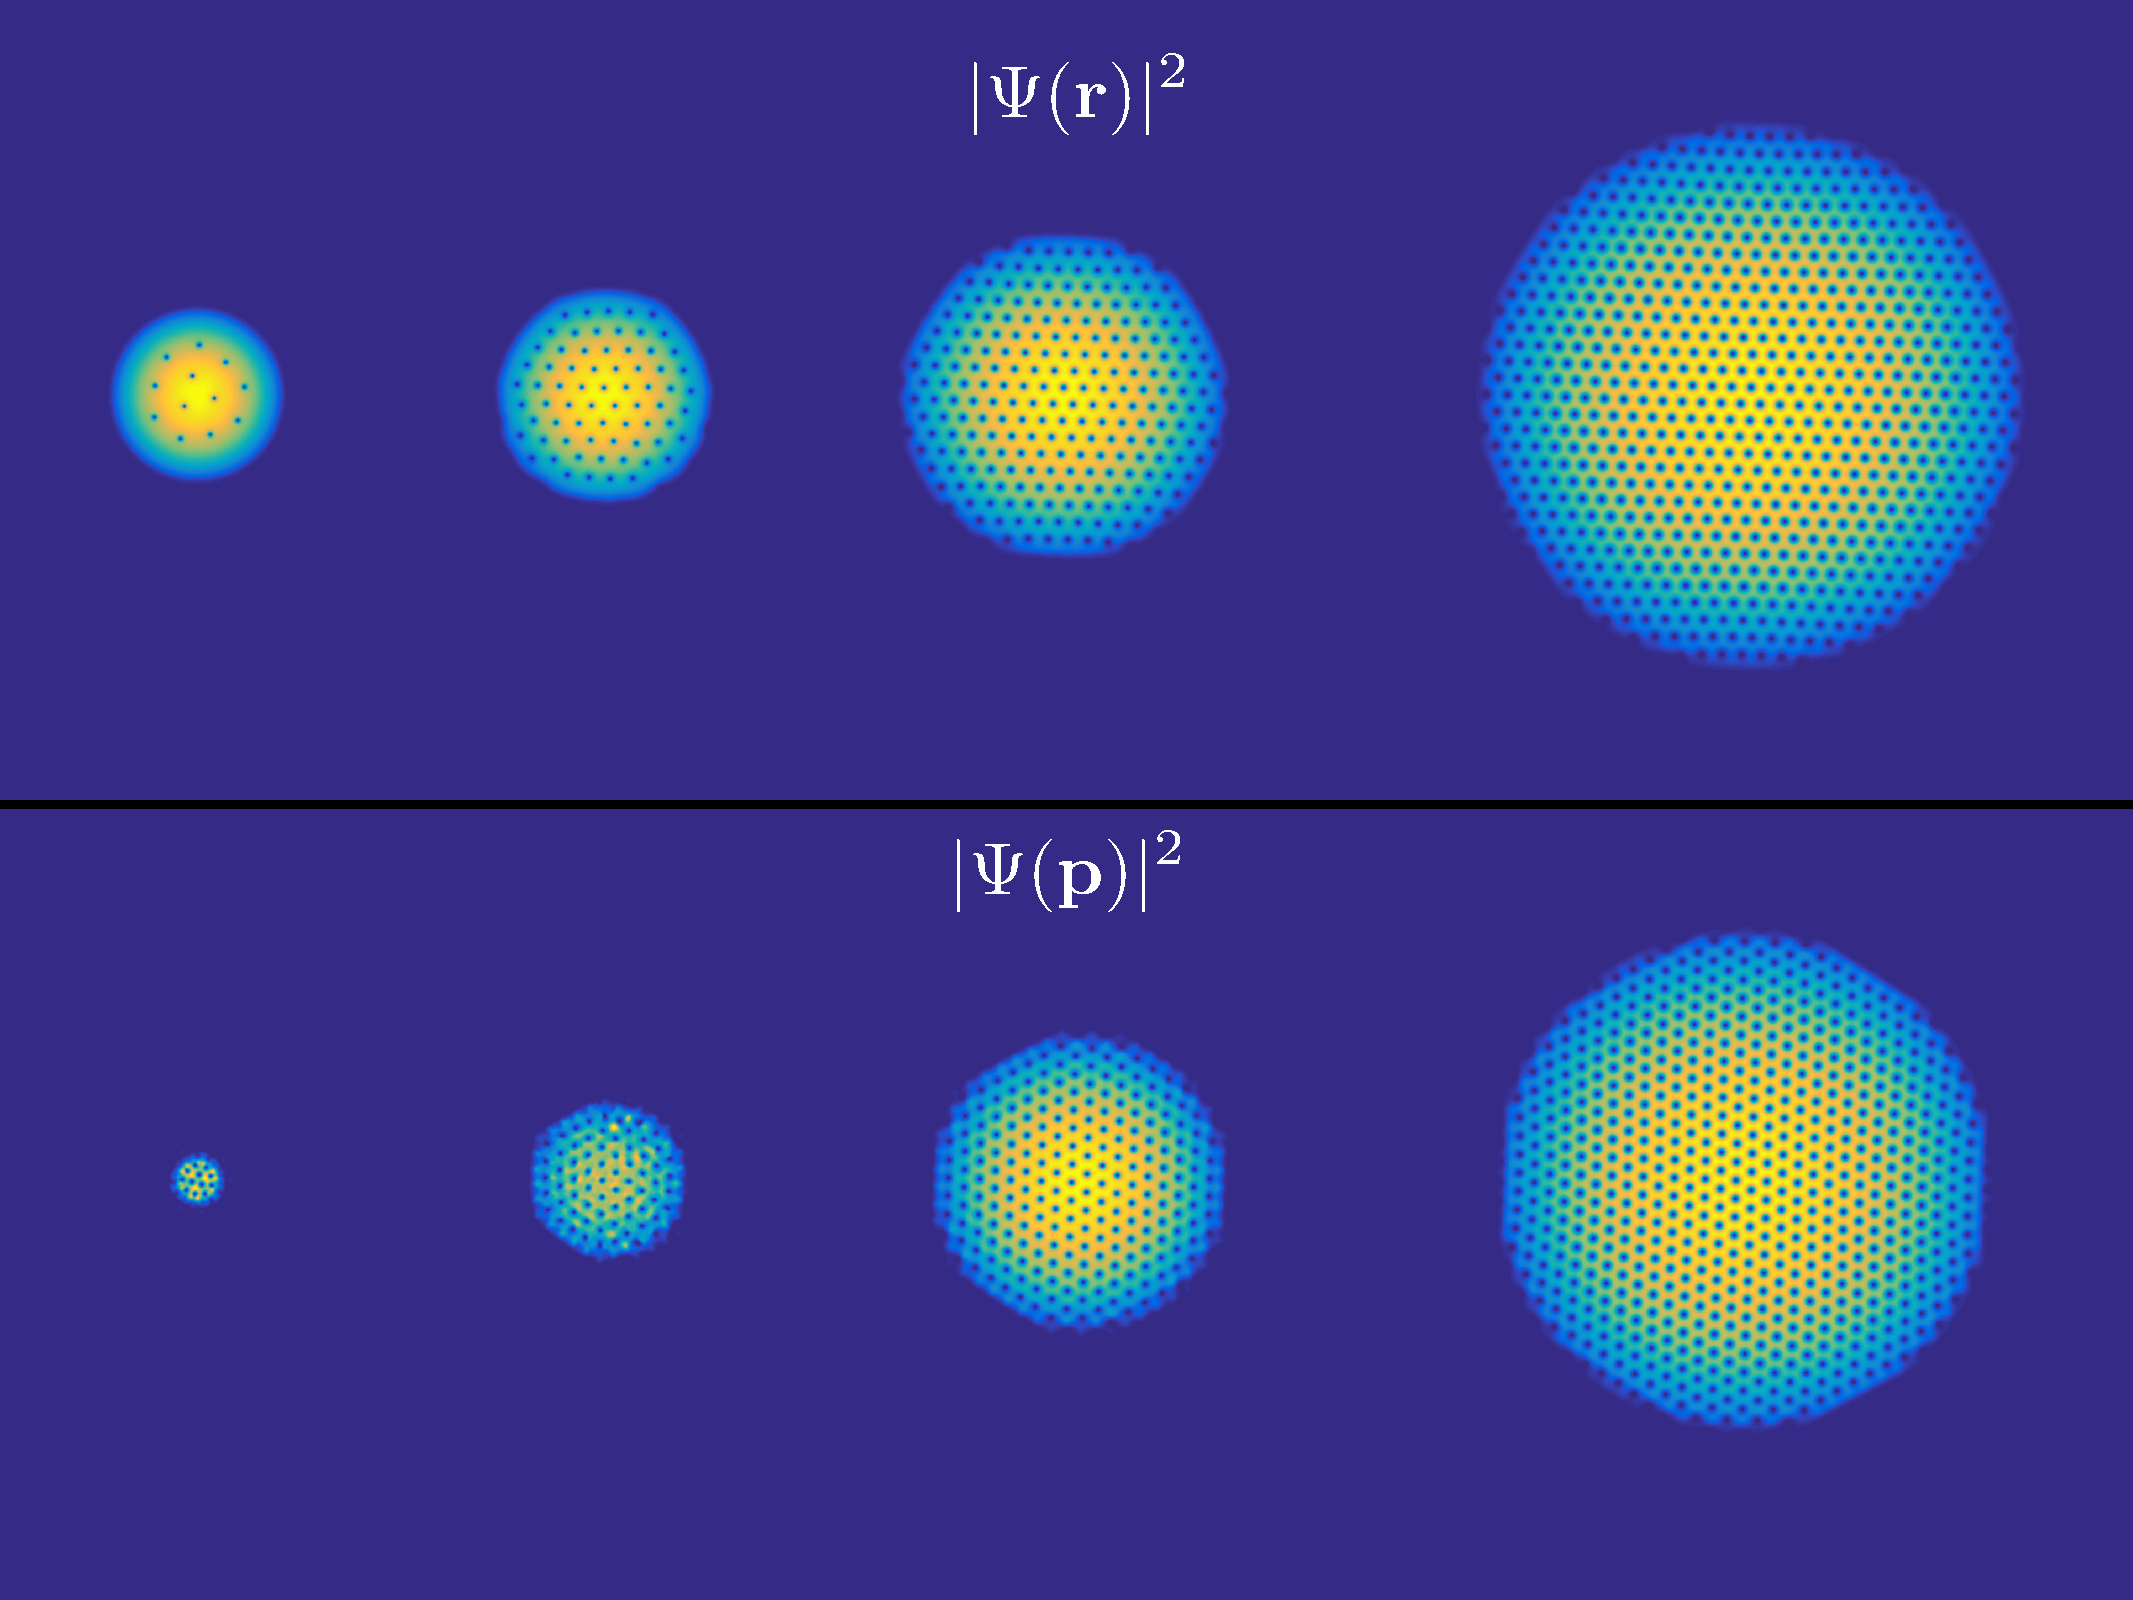
\includegraphics[width=0.85\textwidth]{Images/ch4_vtx/ramp_omega.pdf}
    \caption{If the rotation frequency is chosen at $\Omega=0.995\omega_\perp$ without allowing the lattice to form and order, the resulting vortices all enter instantaneously and compete for position. !!!!}
    \label{fig:malformed_lattice}
\end{figure}

\section{Rapidly rotating vortex lattice}
Given the need for a well ordered vortex lattice it is instructive to discuss the generation of such a system. I assume an initial wavefunction guess of a two-dimensional gaussian having some finite overlap with the groundstate of the system in the absence of angular rotation. Following an imaginary time-evolution like what was outlined in Sec.~\ref{sec:numerics}, the groundstate of the condensate is found.


\subsection{Gaussian phase}

\subsubsection{One dimensional}

\subsubsection{Two dimensional}



\section{Few vortex states}
As discussed in Section~\ref{sec:superfluid}, the discovery and manipulation of quantum vortices remains an active area of research.


Given that the energy of a vortex-carrying condensate scales as $E\propto l^2$, as $L_z \propto l$, any increase in the angular momentum causes a squared increase in the energy. Thus, for energetic favorability, the system prefers to maintain singly-charged vortices. To generate a vortex in the condensate costs energy,

Wi

\section{Quantum vortex dynamics}



\section{Vortex lattice states}
    \begin{equation}
        E(\Psi) = \int \Psi^{*} H_{\text GP} -\Omega L_z \Psi
    \end{equation}





\subsection{Trapping potential control}
A system modelled by the GPE Hamiltonian, $H_{\textrm{GP}} = \left[-\frac{\hbar^2}{2m}\nabla^2 + V(\textbf{r}) + g\vert\Psi(\textbf{r},t)\vert^2 \right]$ Eq.~\ref{eqn:h_gp} allows for a numerically evaluated ground-state. Let us now imagine an abrupt change to this Hamiltonian, such that, $H = H_{\textrm{GP}} + f(t) V_{\textrm{ext}}$, where  $V_{\textrm{ext}}$ is an arbitrary external potential, and $f(t)$ is some function of time to control the application of $V_{\textrm{ext}}$ . In this scenario, the wavefunction, formerly a stationary state of $H_{\textrm{GP}}$, will no longer remain so in the new Hamiltonian provided that $H_{\textrm{GP}} $ and $f(t) V_{\textrm{ext}}$ are non-commuting. Any modification of the Hamiltonian in this way can be viewed as a method for changing the phase of the resulting wavefunction, assuming the time of application of the additional term is much shorter than the timescale of condensate dynamics.
%\begin{equation}
%    e^{i\phi} \mapsto \exp\left(-i\frac{Ht}{\hbar}\right),
%\end{equation}

\begin{subequations}
\begin{align}
    \Psi_0 &= |\Psi_0|e^{i\theta_0} \\
    \Psi(t) &= \Psi_0 e^{-\frac{i H t}{\hbar}} \\
    \Psi(t) &= |\Psi_0| e^{i\left(\theta_0 - \frac{H t}{\hbar}\right)} \\
    \theta^{'} &= \theta_0 - \frac{H t}{\hbar}
\end{align}
\end{subequations}
wherein I have made use of Eq.~\ref{eqn:madelung}. By modifying the Hamiltonian the resulting components of the wavefunction see a different phase which governs their evolution. One common means to manipulate the Hamiltonian is through the use of optical potentials, which can be adjusted and manipulated through a variety of ways. An arbitrary optical field, described by a wavevector $\mathbf{k}$, and frequency, $\omega$ is given by
\begin{equation}
    E(\mathbf{r},t) = \alpha e^{\textrm{i}\left(\mathbf{k}\cdot\mathbf{r} - \omega t\right)},
\end{equation}
where $\alpha$ is the field amplitude. Assuming counter propagating plane waves, we obtain a standing wave solution of the resulting optical potential as
\begin{equation}
    V_{\textrm{ext}} = \gamma \cos^2 (\mathbf{k} \cdot \mathbf{r})
\end{equation}
where $\gamma$ is the resulting field intensity. The optical potential forms a highly periodic system given an appropriately choosen $\mathbf{k}$, and is known as an \textit{optical lattice}. Optical lattices have become very prolific in BEC experiments, with experimental control being very highly developed.

The optical lattice potential can be used to create one, two, or three-dimensional periodic trapping structures. This is achieved by the summation of additional lattice potentials with wavevectors $\mathbf{k}_{1,..,n}$. To create a lattice with $n$-fold rotational symmetry requires $n/2$ $\mathbf{k}$-vectors separated by $\frac{2\pi}{n}$, and that $n/2 \in \mathbb{Z}^{+}$. Taking a square lattice as an example, it has 4-fold rotational symmetry, giving a requirement of two $\mathbf{k}$-vectors, separated by $\pi/2$, as
\begin{equation}
    \mathbf{k} =
    \begin{bmatrix}
     1 & 0 \\
     0 & 1
    \end{bmatrix}.\label{eqn:sqlatt}
\end{equation}
The resulting two-dimensional square lattice potential is shown in Fig.~\ref{fig:cos2xy}.
\begin{figure}[tb]\centering
    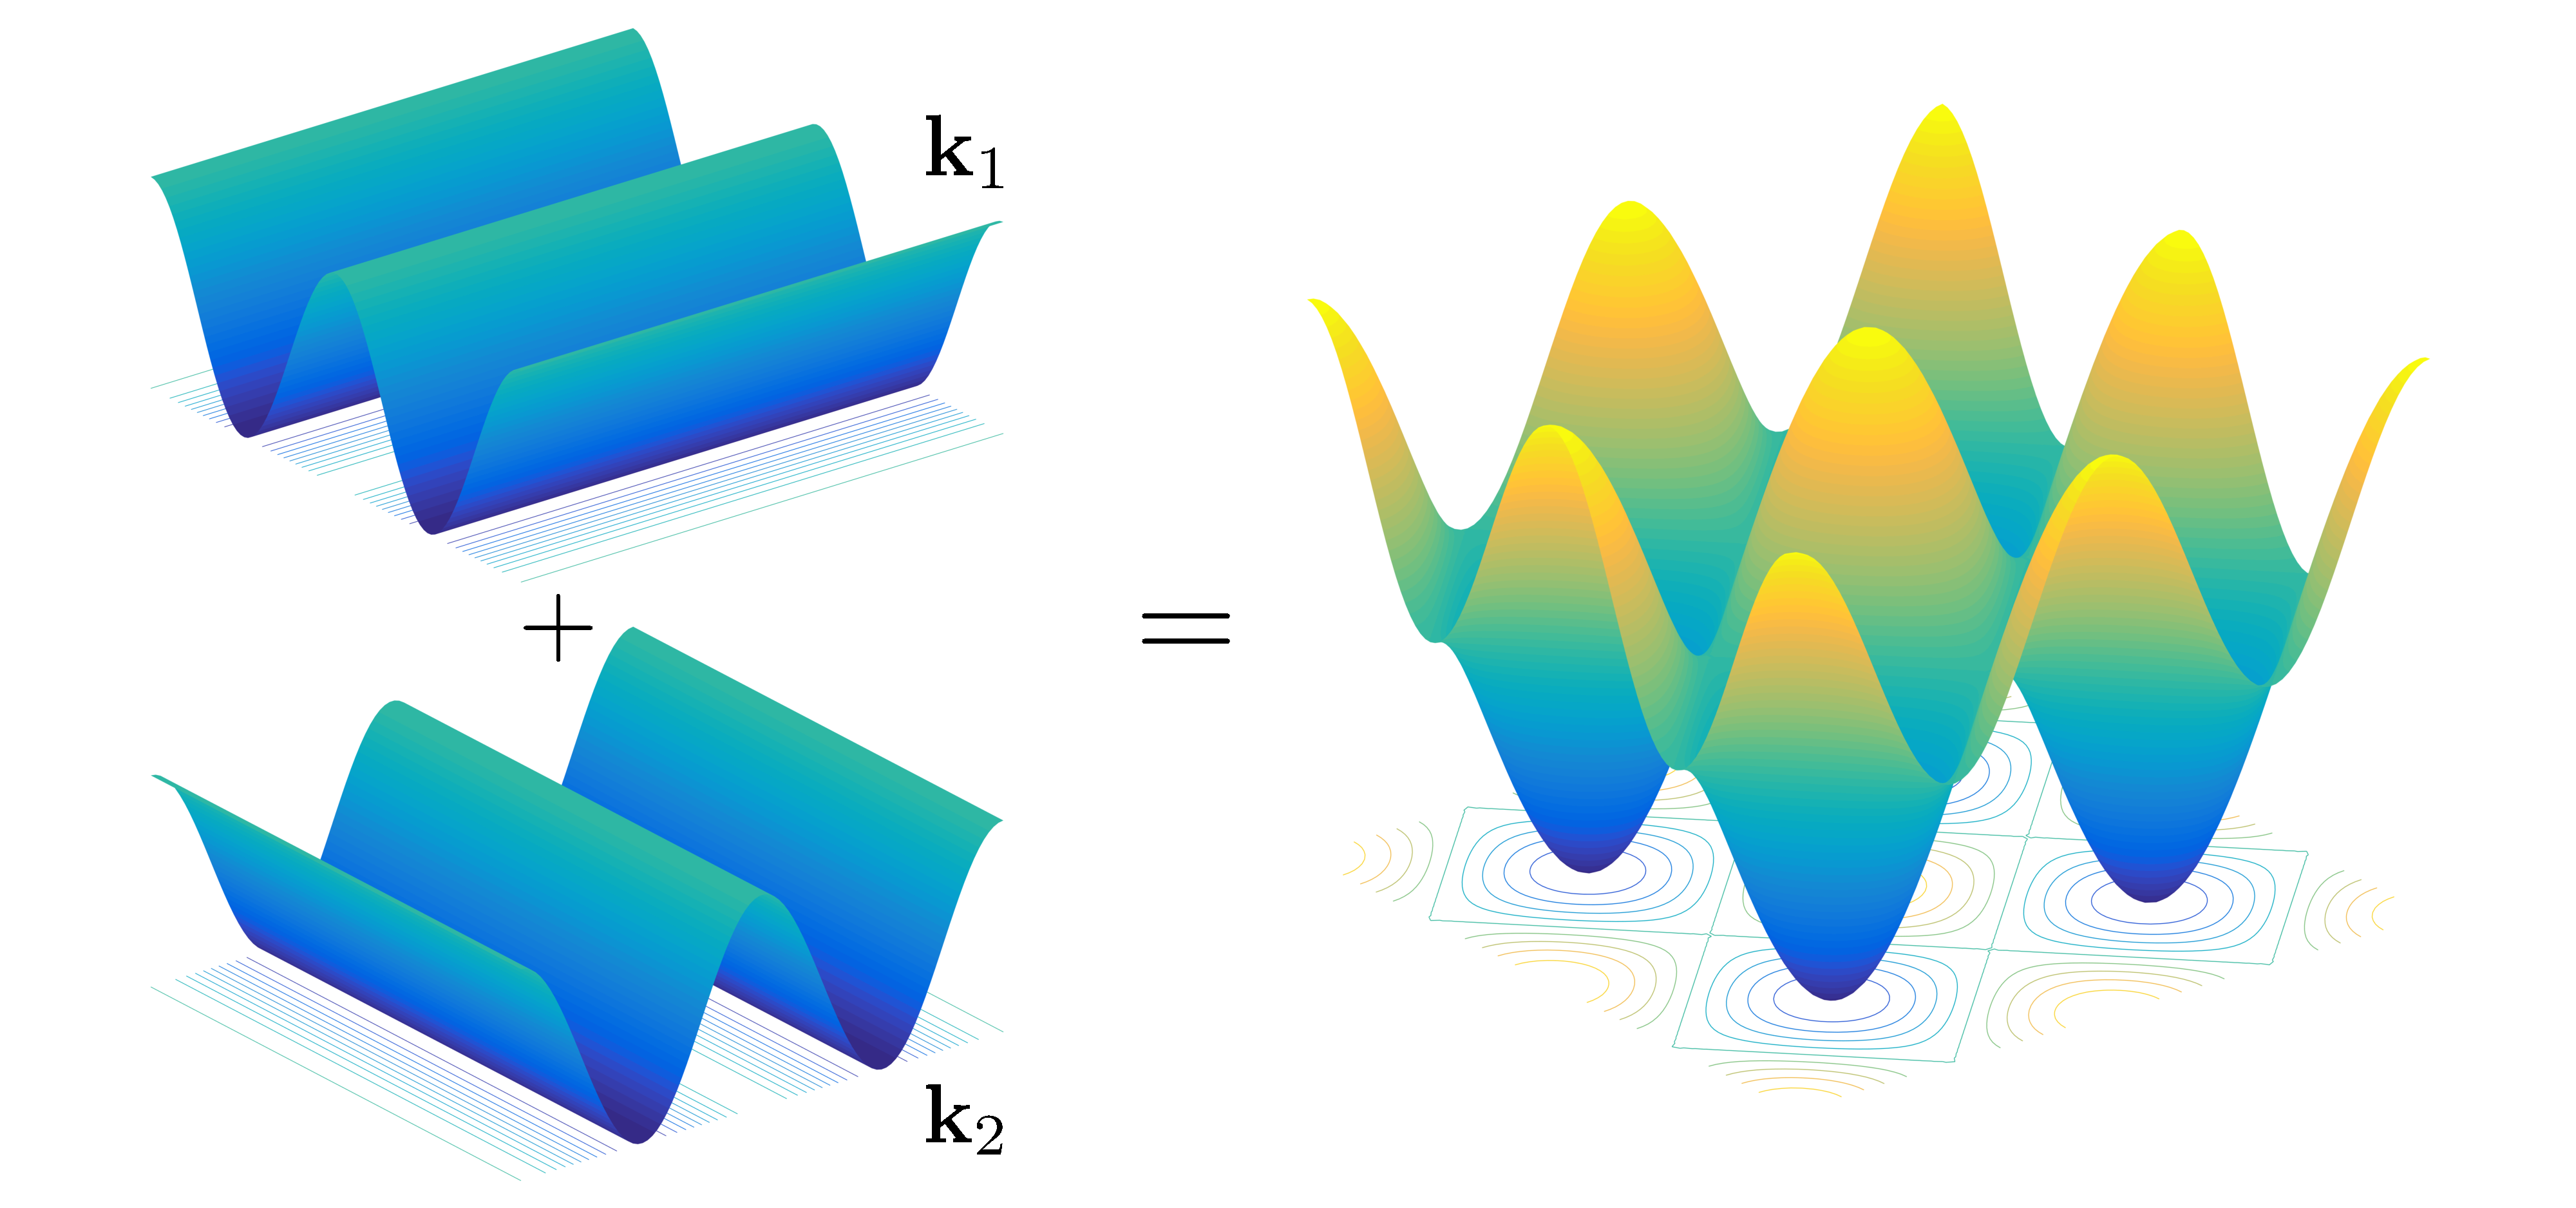
\includegraphics[width=0.55\textwidth]{./Images/ch4_vtx/VOPT/squarelatt}
    \caption{Square lattice generation using two orthogonal propagating laser fields, as defined by Eq.~\ref{eqn:sqlatt}.}\label{fig:cos2xy}
\end{figure}

For the purpose of my system, I intend to create a two-dimensional optical lattice, wherein the structure of the lattice matches that of the triangular Abrikosov vortex pattern. The triangular lattice has 6-fold rotational symmetry, and can be formed with wavevectors

\begin{subequations}
    \begin{align}
        \mathbf{k}_1 &= k_0\left\{\frac{\sqrt(3)}{2},\frac{1}{2}\right\} \\
        \mathbf{k}_2 &= k_0\{0,1\} \\
        \mathbf{k}_3 &= k_0\left\{\frac{\sqrt(3)}{2},-\frac{1}{2}\right\} \\
    \end{align}
\end{subequations}
where $k_0 = 4\pi/(\sqrt(3)a_0)$, and $a_0$ is the lattice spacing.


By choice of $f(t)$, the time of application of the optical lattice to the condensate can be controlled. Given some time for evolution, the wavefunction phase will be modified and evolve due to the presence of the new potential. Of particular interest is the use of an instantaneously switched optical potential. For an optical lattice that is switched on and permanently remains on, such as $f(t) = \Theta(t)$ where $\Theta$ is the Heaviside step function, the condensate will see this as a quench, and attempt to adjust to the new Hamiltonian. However, for a pulsed optical lattice, such as a $\delta$-function in time, the condensate responds as though it receives a kick, with the resulting kick modifying the phase profile of the wavefunction. Experimentally, one can imagine this effect coming from the use of an optical shutter, and thus we can assume this is a realisable perturbation, with the potential intensity controlled by beam power.


\iffalse
The resulting intensity pattern is given by
\begin{equation}
    I = | \Re{E} \Re{E^{*}}| = \gamma \cos^2 (\mathbf{k} \cdot \mathbf{r} - \omega t),
\end{equation}
with $\gamma = \alpha\alpha^{*}$ as the intensity amplitude. If one assumes the field describes a wave propagating along $\mathbf{k}$, a standing wave pattern can be formed by counter-propagation of the same field along $-\mathbf{k}$.  The resulting field intensity is given by
\begin{equation}
    I_{sw} = \Gamma \cos^2 (\mathbf{k} \cdot \mathbf{r})\cos( \omega t)
\end{equation}
where the intensity of the fields are stationary along $x$, and the amplitudes oscillate in time at a rate $\omega$. The dipole force experienced by an atom is directly proportional to the gradient of the intensity, $\mathbf{F} \propto -\nabla I_{sw}$. By assuming the rotating wave-approximation, where we rotate at the rate of the laser field, we obtain a time-dependent optical potential, given by
\begin{equation}
    I_{sw} = \Gamma \cos^2 (\mathbf{k} \cdot \mathbf{r})\cos( \omega t)
\end{equation}
\fi
\iffalse
An arbitrary set of optical fields can be given by
\begin{equation}\label{eqn:optfield}
    f_{\textrm{P}} = \displaystyle\sum\limits_{j} \alpha_j e^{\textrm{i}\left(\mathbf{k}_j\cdot\mathbf{r} - \omega t\right)},
\end{equation}
where $j$ is the row index of the individual optical field, $\alpha_j$ is the amplitude of the field, $\mathbf{k}_j$ is the respective wavevector, and $\omega$ is the oscillation frequency of the wave. By careful choice of $\alpha$ and $\mathbf{k}$ any arbitrary potential geometry can be formed through Fourier synthesis. For the purpose of my system this may reduced through several simplifications, resulting in what remains as a realistic system. Given that an explicit time-dependence on the potentials would introduce experimental difficulties, one can assume that for the cases examined herein that the optical fields are time independent (i.e $\omega=0$), and are counter-propagating plane waves. This reduces the summation to a linear combination of cosine terms. Lastly, as I only require the intensity for defining the potential geometry, the corresponding optical potential can be written as
\begin{equation}\label{eqn:vopt}
    V_{\textrm{O}} = \displaystyle\sum\limits_{j} \gamma_j \cos^2 \left(\mathbf{k}_j \mathbf{r}\right),
\end{equation}
where $\gamma$ is the amplitude of the individual potential components. By choosing the values of $\mathbf{k}_j$ to match the lattice vectors of a required lattice geometry, the optical potential may take this form. For the work described herein I restrict the dynamics to two-dimensions. Fig.~\ref{fig:squarelatt} demonstrates this with a square lattice geometry, given by
\begin{equation}\label{eqn:sqlatt}
    \mathbf{k} =
    \begin{bmatrix}
     1 & 0 \\
     0 & 1
    \end{bmatrix} =
    \begin{bmatrix}
     \mathbf{k}_1  \\
     \mathbf{k}_2
    \end{bmatrix}.
\end{equation}
\fi

%%%%%%%%%%%%%%%%%%%%%%%%%%%%%%%%%%%%%%%%%%%%%%%%%%%%%%%%%%%%
\subsection{Direct phase manipulation}\label{sec:phase}
%%%%%%%%%%%%%%%%%%%%%%%%%%%%%%%%%%%%%%%%%%%%%%%%%%%%%%%%%%%%%%%%%%%%%%%%%%%%%%%%%%%%%%%%%%%%%%%%%%%%%%%%%%%%%%%%%%%%%%%%%%%%%%%%%%%%%%%%%%%%%

While groundstate condensates will have a flat phase across the system, there are some interesting examples where a spatially dependent phase exists: dark solitons and vortices. I have previously discussed the $2\pi$ phase profile of a vortex. Dark solitons are another type of topological excitation that feature a $\pi$ jump phase profile. These excitations are unstable dimensions higher than one, and will decay via a snake instability to vortices [citation].

Where previously I have considered the evolution of the wavefunction in the presence of a kicked smoothly varying optical potential, one can also consider the case of a directly imprinted phase. Phase imprinting is a technique that applies a spatially inhomogeneous potential across a condensate in such a way that the phase is modified to a desired form. As a consequence the density distribution will adjust itself in time and dark solitons \cite{BEC:Denschlag_science_2000}, as well as vortices \cite{Vtx:Dobrek_pra_1999} have been created this way. For the latter the signature is given by a phase singularity, around which the phase winds through $\pm 2\pi$, depending upon the direction of rotation. As discussed in Sec.~\ref{sec:}, this is the phase profile given for a quantum vortex, and by application of this pattern one can create such a topological defect in the wavefunction.

Following \cite{BK:Pitaevskii_Stringari_2003} and taking the Madelung transform of the wavefunction given by Eq. \eqref{eqn:madelung}, the phase of the condensate may be specified as
\begin{equation}
\theta = \theta^{(c)} + \theta^{(i)},
\end{equation}
where $\theta^{(c)}$ is the unperturbed condensate phase, and $\theta^{(i)}$ is the phase pattern to be imprinted. Usually $\theta^{(c)}$ is constant allowing the simple addition of features such as vortices and solitons to a condensate wavefunction. Thus, upon solving for the initial condensate phase, an additional phase pattern can be imprinted at any time by multiplying the wavefunction by $e^{i\theta^{(i)}}$. More generally, without careful choice of the phase terms their addition can lead to a mess, so care must be taken to choose a well defined initial and imprinting phase pattern.

Where previously I added an optical potential to the Hamiltonian for a short time during the evolution, here I directly engineer the wavefunction phase. Though the same desired effect is performed physically with that of the previously discussed optical lattice potential, I now model the application of the phase by directly controlling the wavefunction itself. The advantage of the phase imprinting model is that for topological defects, one can essentially imprint the required winding instantaneously. The density also need only adjust itself local to the phase singularity, with the remaining condensate seeing an almost constant shift in phase.

The creation of vortices through application of localised $\pm 2\pi$ phase winding defects in the condensate allows for direct control of the vorticity and angular momentum of the BEC. Given the rapid change of the phase, and hence the kinetic energy of the condensate, the appearance of phonons are expected following the imprint. While it has been discussed in the literature for creation of vortices, the phase imprinting method can also be used to annihilate a vortex from the condensate by applying a phase profile of opposite winding, removing the singularity. This will leave the condensate with a density depletion at the prior location of the phase singularity. Without the singularity this depletion will fill in and excite phonon modes in the condensate during time evolution. This method will form the basis for which the further discussions and analysis are performed on the vortex carrying condensate.

Experimental realisation of arbitrary phase patterns are accessible through the use of spatial light modulators (SLM). These devices behave as digital monitors, through which any visual pattern can be expressed, allowing the masking of a laser field to the required form. I will assume for all future discussions that the potentials are experimentally realisable, and focus on the resulting effect on the condensate. For the creation of a single vortex the $2\pi$ phase winding pattern can be created spatially using
\begin{equation}
    \phi(\mathbf{x},\mathbf{y},x_0,y_0) = \atantwo(\mathbf{y}-y_0,\mathbf{x}-x_0),
\end{equation}
where the singularity is located at the position $\left(x_0,y_0\right)$. The resulting phase is shown by Fig.~\ref{fig:atan2phase}.
\begin{figure}\centering
    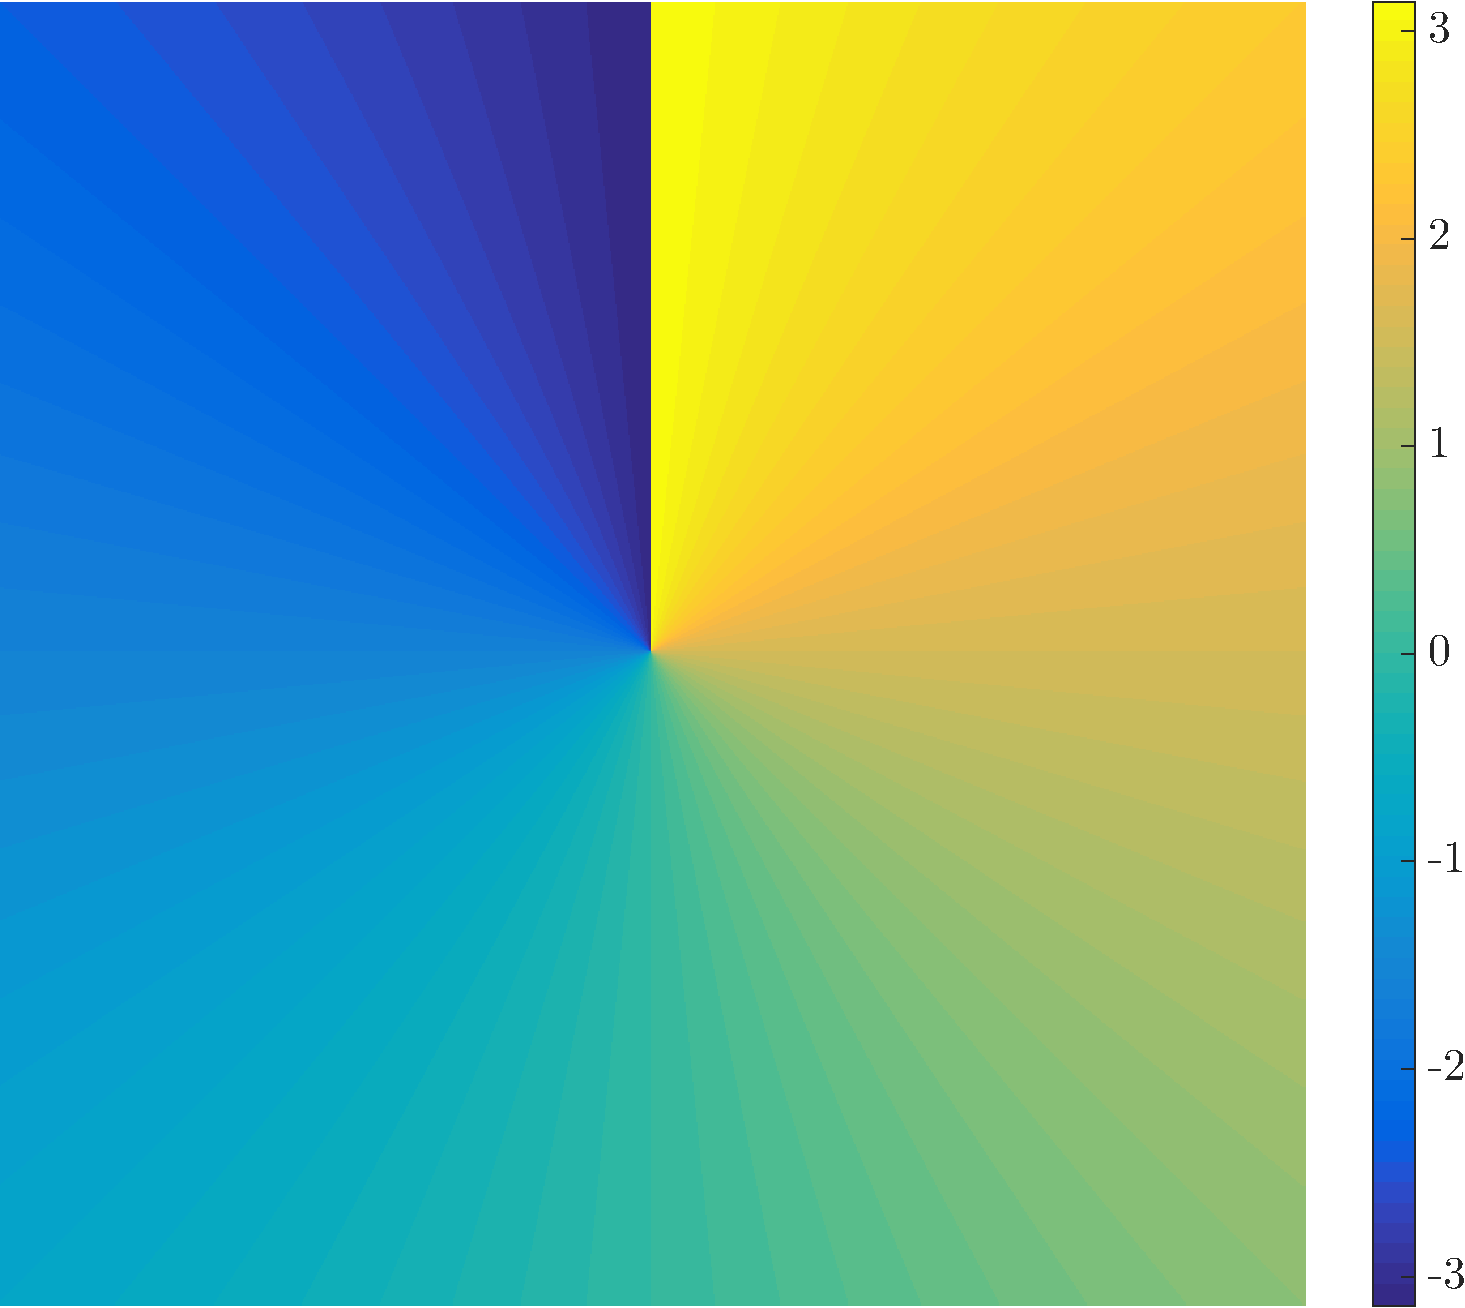
\includegraphics[width=0.45\textwidth]{Images/ch4_vtx/2pi.pdf}
    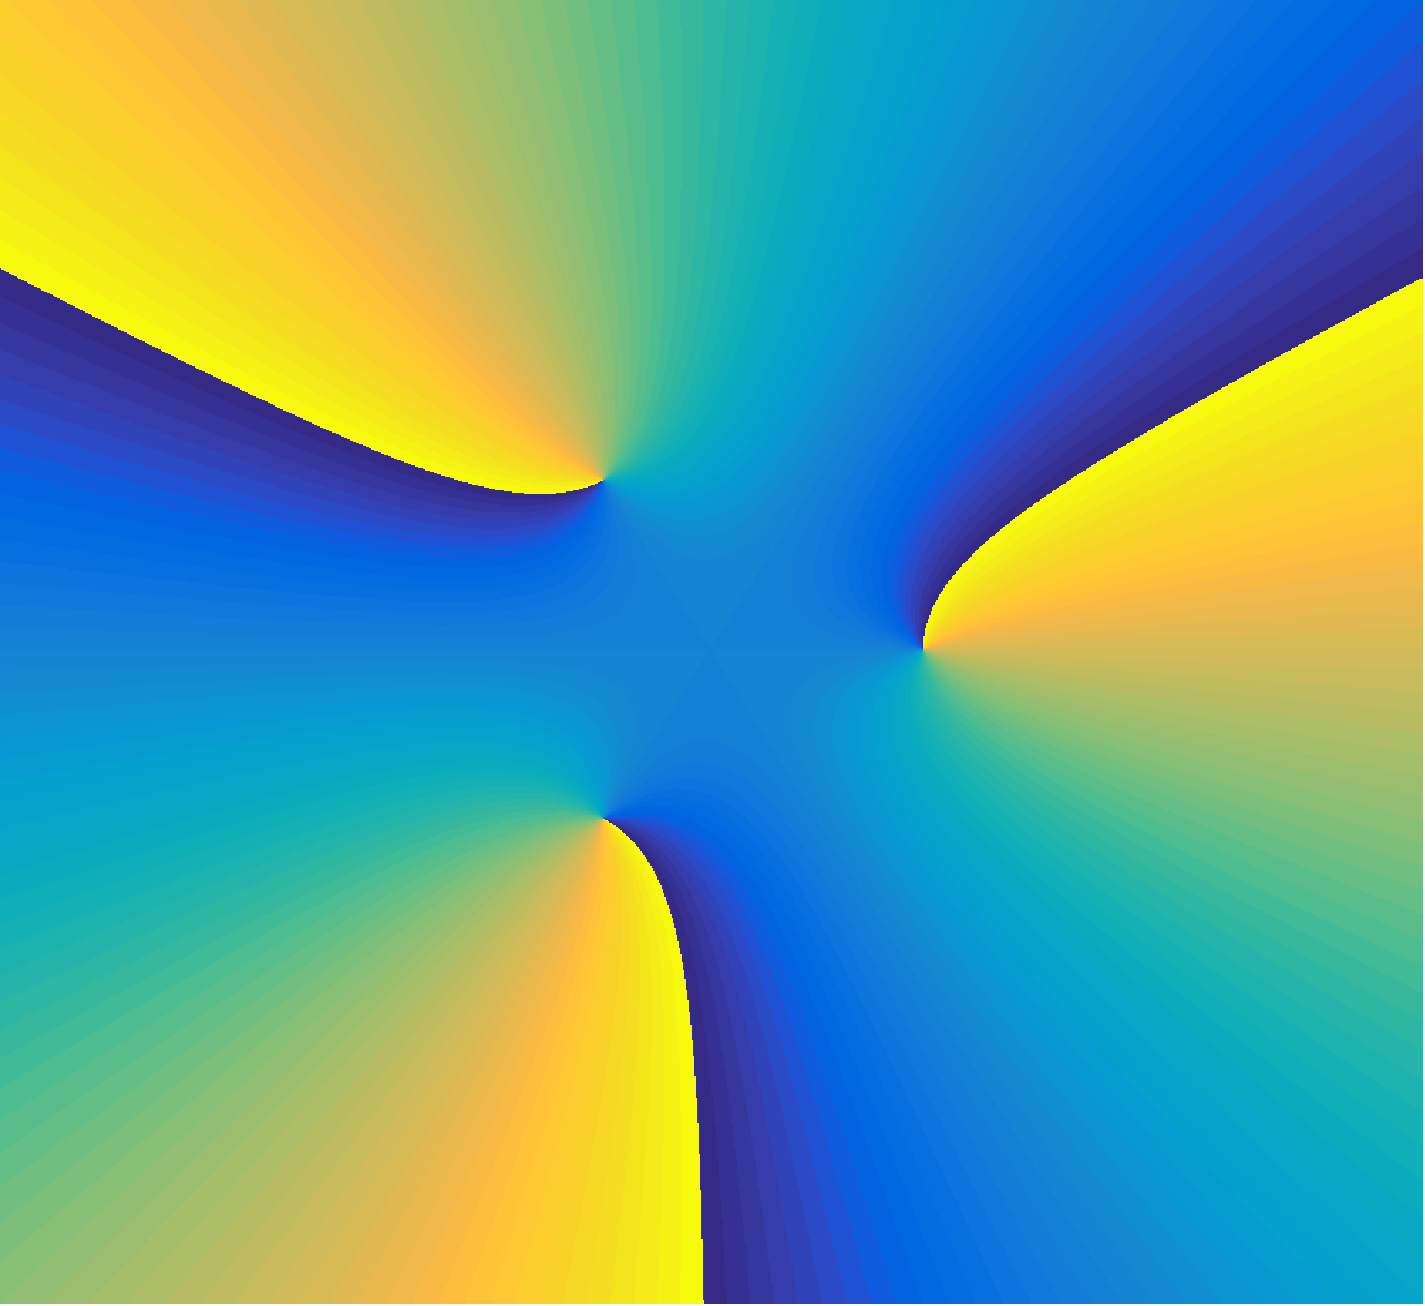
\includegraphics[width=0.435\textwidth]{Images/ch4_vtx/3_2pi.pdf}
    \caption{The $2\pi$ phase winding is shown for a single (left) and three separated (right) defects. The application of separate phase singularities can be treated as summing each individual phase profile, $\displaystyle\sum\limits_i \theta_i \mod 2\pi$.}\label{fig:atan2phase}
\end{figure}

Writing the wavefunction in the standard Madelung transform form, and including the additional phase singularity term $\theta_i$, I imprint this singularity to the condensate wavefunction as
\begin{equation}
    \Psi(\mathbf{r},t) = |\Psi(\mathbf{r},t)|e^{\text{i}(\theta_c(\mathbf{r},t) + \theta_i(\mathbf{r}))}.
\end{equation}
An example of this is given in Fig.~\ref{fig:0to1vtx}, where the condensate density and phase is shown, following imaginary time evolution, before and after a phase imprint.

\begin{figure}\centering
    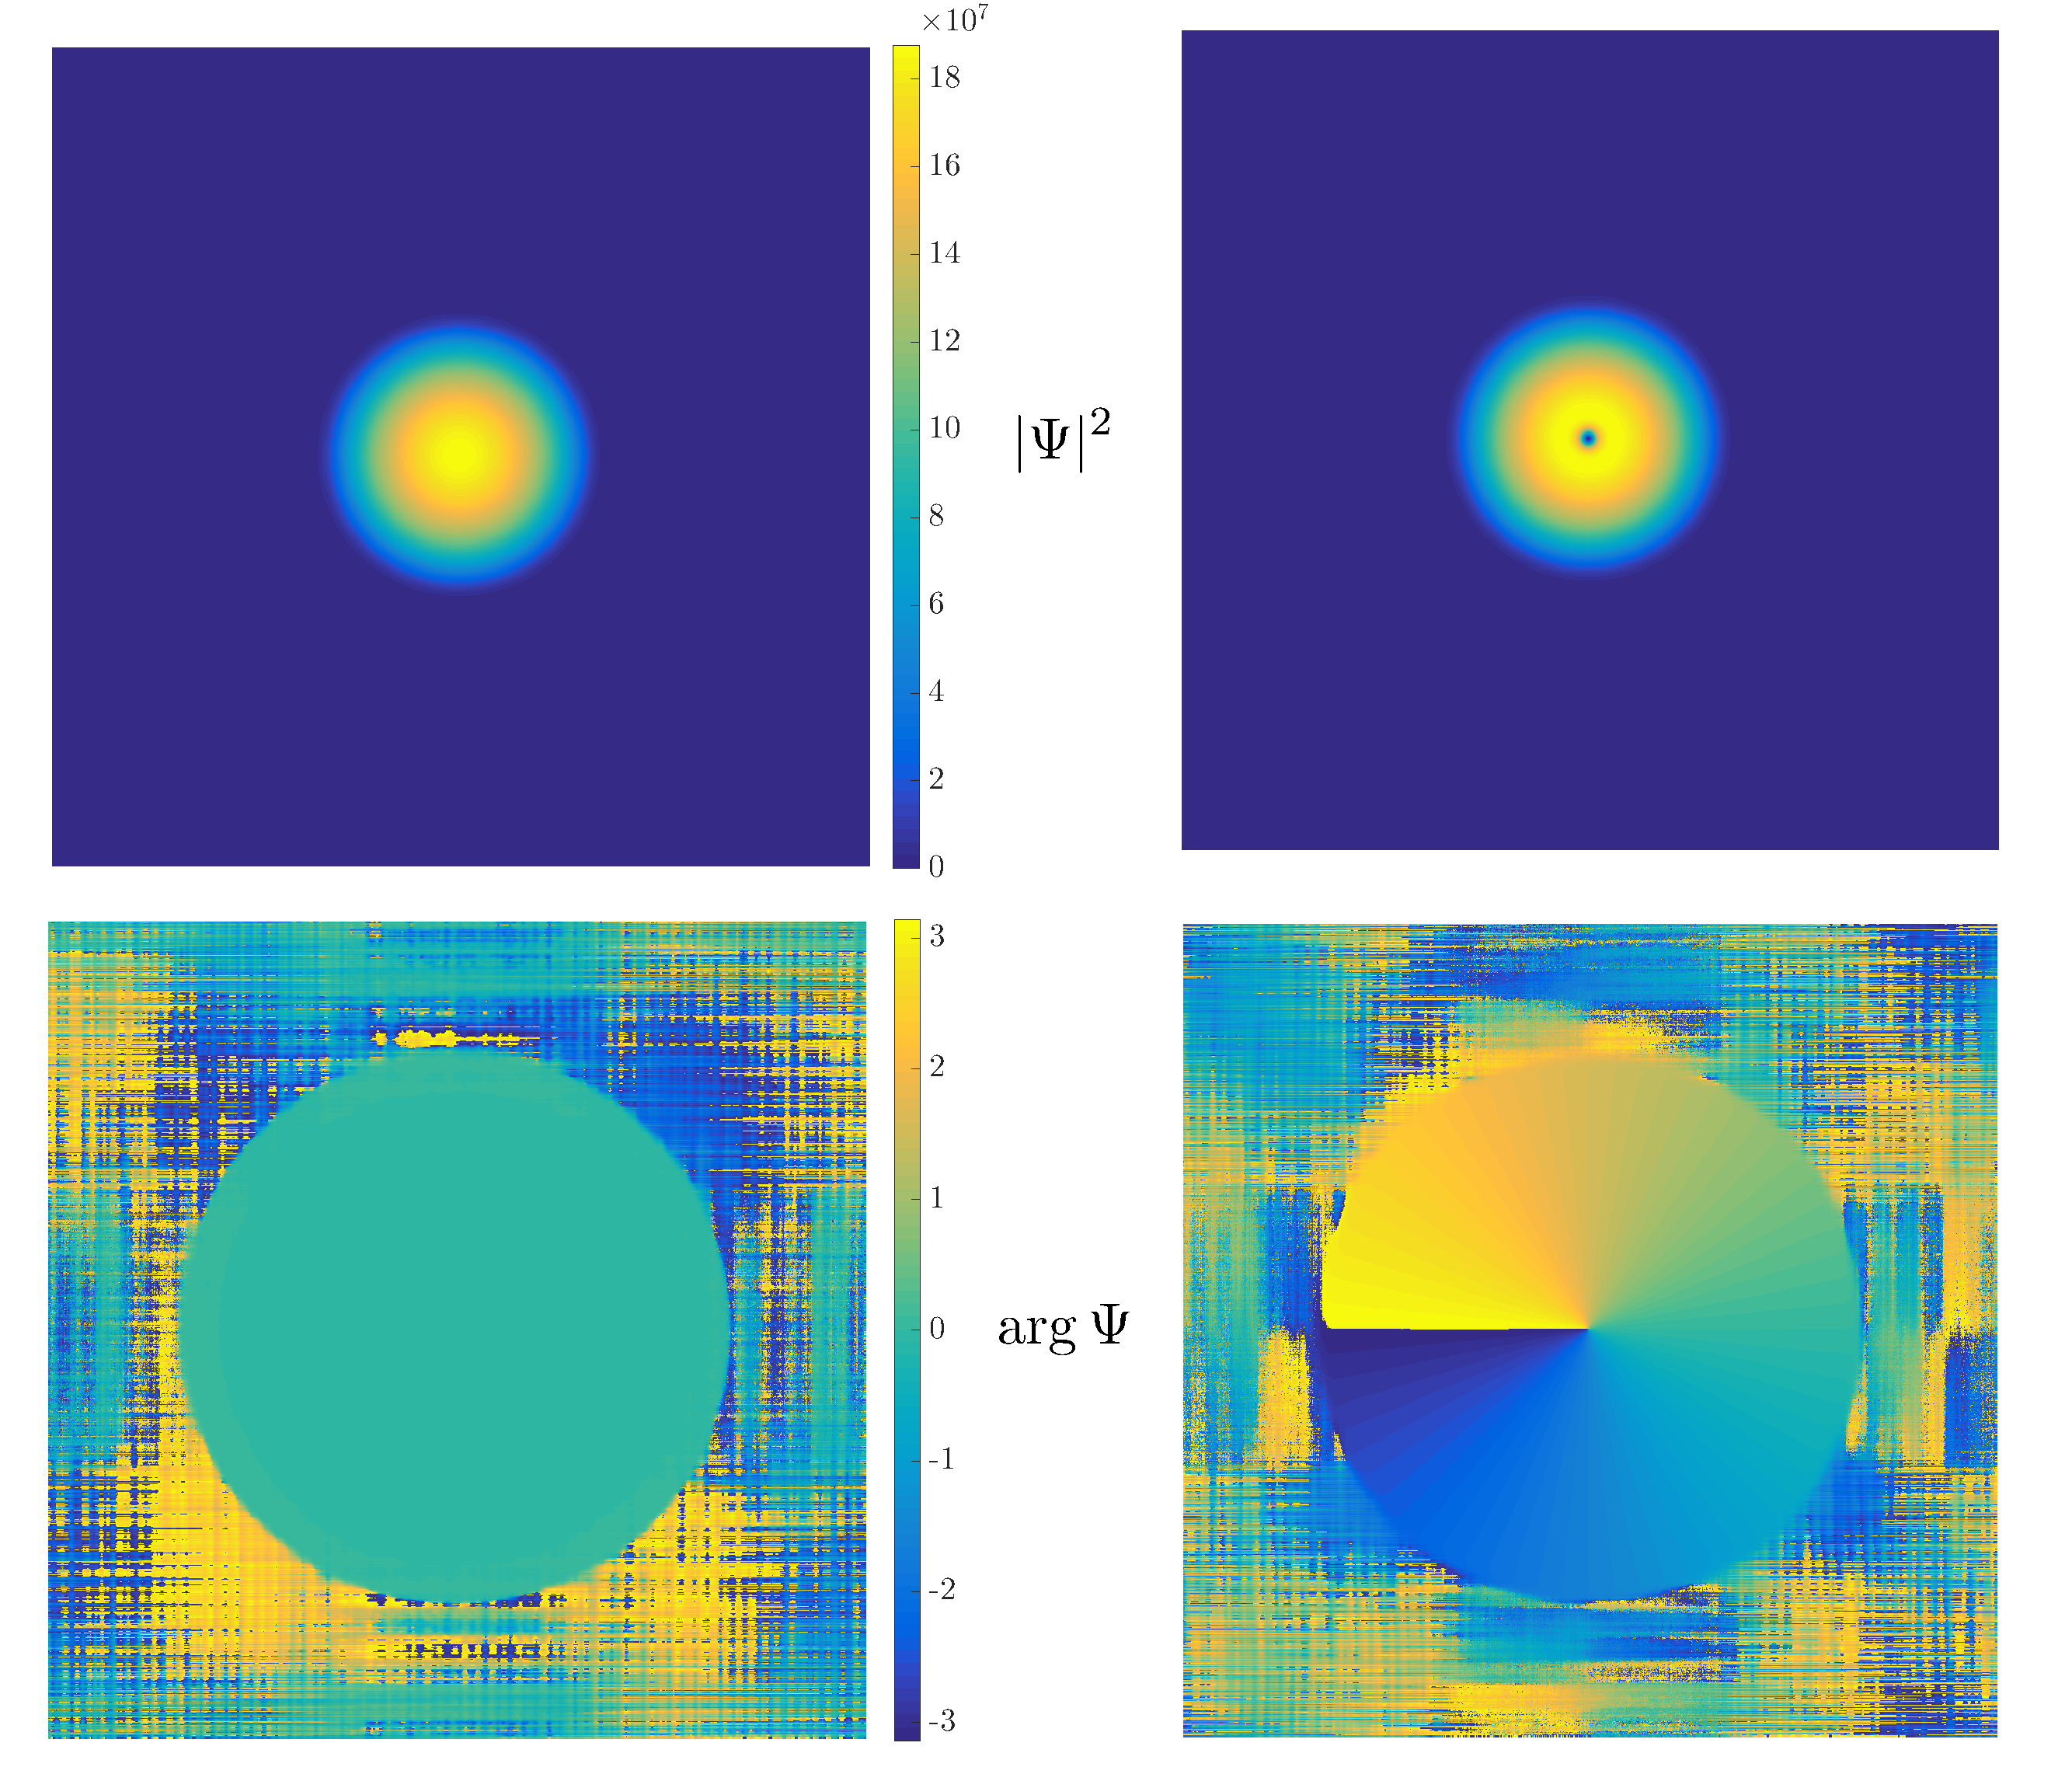
\includegraphics[width=0.75\textwidth]{Images/ch4_vtx/1vtxbec.pdf}
    \caption{The condensate density and phase are shown in the absence and presence of a vortex. The density dip location corresponds exactly with the phase singularity, around which it winds from $-\pi$ to $\pi$}.\label{fig:0to1vtx}
\end{figure}
While here I have shown the creation of a groundstate solution with the phase imprint and imaginary time evolution, this process may also be carried out during real-time evolution. For a closed system the vortex imprint will raise the energy of the system, and likely not be a groundstate.
